To achieve our objective of building a spanning tree that minimizes the distances between all
connected pair of nodes in the original graph, we rely on a particular subgraph structure, namely
the star.  We therefore introduce two algorithmic primitives: \extractStar{}, which partition a
graph $G$ into a set of disjoint stars; and \collapseStar{}, which selects edges from $E$ to
assemble these stars into a new, smaller graph. Given a graph topology $G_0=(V_0, E_0)$ and assuming
for simplicity that $G_0$ consists of a single connected component,\footnote{For we can otherwise
run our algorithm in parallel on each connected components of $G_0$.} the \gtx{} algorithm
repeatedly applies these two primitives to produce a sequence of graphs $\{G_t\}_{t=0}^K$ of
decreasing size, until $G_K$ is made of a single node. All the edges selected while reaching
this stage then form the spanning tree we were looking for.
This can be seen as a simple instantiation of a general procedure described in \autocite[Section
5.2]{LowerBound95}.
% [from a CMU NIPS submission http://www.stat.cmu.edu/~arinaldo/papers/mutualfriends.pdf] We
% consider Mutual-Friends to be *an algorithmic primitive*, by which we mean a kind of subroutine for
% a more complicated function that iterates Mutual-Friends, similarly to [5].

In the following, we provide a more precise description of our two primitives and analyze their
complexity. Then we state formally the complete \gtx{} algorithm, prove its termination and
correctness, and show a detailed example of its execution.  Finally, we study its properties, such
as the number of iterations needed to finish and the stretch of the resulting tree.

\paragraph{\extractStar{}}\label{par:extractstar}%
\extractStar{} takes as input a graph $G_t=(V_t, E_t)$.
While the nodeset $V_t$ is not exhausted, it repeatedly samples a
node $c_i$, creates a star $S_i^t$ with $c_i$ at its center and the neighbors of $c_i$ on the
periphery, removes all the nodes of $S_i^t$ from
$V_t$ and all the edges incident to $S_i^t$ from $E_t$, and finally decrements accordingly the
degree of the 2-hop neighbors of $c_i$ (see \autoref{fig:gtx_star_simple} for a visual
representation of this notation).
Upon completion, it returns a list of stars,
the set of all the edges within a star,
and a map (or associative array) that associates each node of $V_t$ to the index of the
unique star it belongs to.
According to the definition of \textcite{HashTableBook08}, an associative array is an abstract data
type composed of a collection of (key, value) pairs, such that each possible key appears at most
once in the collection. It efficiently supports the addition, removal and modification of a pair, as
well as the lookup of a value associated with a particular key.
\begin{marginfigure}
  \centering
  \includegraphics[height=0.15\textheight]{assets/tikz/gtx_star_tikz.pdf}
  \caption[A sample star]{A sample star created during the \tth{} collapse level. The black node
    % \tikz{\node[vertex,rare] {$c_i$};}
    is the center $c_i$ of the star $S_i^t$, which is also made of the four light gray peripheral nodes
  % \tikz{\node[vertex,medium] {$p_1$};} to \tikz{\node[vertex,medium] {$p_4$};}
  as well as the solid edges. The 2-hops neighbors of $c_i$ are the white nodes
  % \tikz{\node[vertex] {$h_1$};} to \tikz{\node[vertex] {$h_3$};}
  $h_1$ to $h_3$, whose degree will decrease once $S_i^t$ is removed from $G_t$.}
  \label{fig:gtx_star_simple}
\end{marginfigure}

As showed in the following pseudo code\footnote{Note that for
clarity, we removed some bookkeeping code in all listings, mainly the part related to maintaining
mapping between nodes at different collapse level. However, the full python implementation
is available at \url{https://github.com/daureg/magnet/blob/master/veverica/new_galaxy.py\#L27}.}, we
sample centers by choosing the node with the current highest degree, with ties broken
arbitrarily.\footnote{We also consider more involved heuristics but, in the interest of simplicity,
they are presented later~\vpageref{ssec:gtx_center_choice}.} This is achieved efficiently by
maintaining a max-priority queue $Q$, initially containing all the nodes of $V_t$. The priority of a
node is its current degree and we equip $Q$ with two standard operations described
by~\textcite[section 6.5]{CormenAlgo09}: \textsc{Extract-Max}$(Q)$ removes and returns the
node of $Q$ with the largest degree and \textsc{Decrease-Key}$(Q$, $u$, $\Delta)$ decrements
the degree of the node $u$ by an amount $\Delta$.
We also assume that $G$ is the adjacency list of the graph, so that $G[u]$ is the set of neighbors of
$u$, \ie{} $G[u] \equiv \mathcal{N}(u)$. Finally $membership$ is a map and we
define the \textsc{Star} function, which creates a star given a center $c$, a list $periphery$ of
peripheral nodes, and a star index $i$. After creating the \ith{} star, for every node $u$ belonging
to that star, the \textsc{Star} function sets $membership[u] = i$.
\vspace{-\baselineskip}

\begin{center}
  \rule{\textwidth}{.3pt}
  \begin{algorithmic}[1]
    \Function{\extractStar{}}{$G_t=(V_t,E_t)$}
      \State Let $Q$ be the max-priority queue described above
      \State Let $remaining$ be a set of nodes, initially containing all the nodes in $V_t$
      \State Let $membership$ be an empty map
      \Let{$stars$}{$[]$}
      \Let{$inner\_edges$}{$\emptyset$}
      \While{$Q$ is not empty}
        \Let{$c$}{\Call{Extract-Max}{$Q$}}
        \If{$c$ not in $remaining$}
          \State \textbf{continue} \Comment{$c$ is part of an existing star so there is
          nothing to do}
        \EndIf
        \Let{$periphery$}{$G_t[c] \bigcap remaining$}
        \Let{$stars$}{$stars \bigcup \{$\Call{Star}{$c$, $periphery$, $|stars|$}\}}
        \Let{$inner\_edges$}{$inner\_edges \bigcup \{(c, p): p \in periphery\}$}
        \Let{$remaining$}{$remaining \setminus \left\{ \{c_i\} \cup periphery\right\}$}
        \For{$p$ in $periphery$}
          \For{$h$ in $G_t[p] \bigcap remaining$}
            \State \Call{Decrease-Key}{$Q$, $h$, $1$}
          \EndFor
        \EndFor
      \EndWhile
      \State \textbf{return} $stars$, $inner\_edges$, $membership$
    \EndFunction
  \end{algorithmic}
  \rule{\textwidth}{.3pt}
\end{center}

\begin{prop}
  \label{prop:gtx_time_extractstar}
  For any connected graph $G=(V,E)$, \extractStar$(G)$ terminates in $O(|E|)$ time.
\end{prop}
\begin{proof}
\extractStar{} terminates because at each iteration of the while loop line 7, we remove one node
from $Q$ and never add any. Let us now analyze its complexity. We first build a priority queue of
all the nodes according to their degree (line 2), which requires $|V|$ insertions into $Q$. Then
we execute $|V|$ iterations of the while loop. However, the main idea here is that we process each
node and each edge exactly once. We first find the center $c$ of the next star by extracting the
maximum of the queue (line 8) and testing if $c$ is still part of the graph, which happens $|V|$
time. Then we build the corresponding star (line 11--14). In total, we test the membership of $|V|$
nodes in line 11, $\textsc{Star}$ updates the $membership$ map $|V|$ times in line 12,
$inner\_edges$ consists of $|E|$ edges at most in line 13 and $remaining$ is only updated $|V|$
times in line 14. Finally, we decrease the priority (\ie{} the degree) of all nodes adjacent to the
new star (line 15--17). Each decrement is supported by a single edge, thus \textsc{Decrease-Keys} is
called at most $|E|$ times. Since all queue operations require constant time when using a Strict
Fibonacci Heap~\autocite{FibonacciHeaps12}, the complexity is $O(|E|+|V|)$, which is also $O(|E|)$
since $G$ is connected.
\end{proof}

\paragraph{\collapseStar{}}\label{par:collapsestar}%

The second primitive, \collapseStar{} takes as input the edges $E_t$ of the current graph, along
with the $membership$ result of \extractStar{} and an $eccentricity$ array. It builds a new graph
$G_{t+1}$ where each star from \extractStar{} becomes a node and where there is a link between two
nodes $s_u$ and $s_v$ if the nodes in $V_t$ making up $s_u$ and $s_v$ are connected in $E_t$. The
$eccentricity$ array is needed because when connecting two stars, we would prefer to join their
center rather than two of their peripheral points. Therefore, we maintain an eccentricity count for
all of the nodes of the original $G_0$, which is incremented by $1$ each time a node is chosen to be
on the periphery of a star. In other words, the eccentricity of an original node quantifies to which
extent it has been pushed to the border of the galaxy.

\begin{marginfigure}
  \centering
  \includegraphics[width=0.92\linewidth]{assets/tikz/gtx_cross_edges_tikz.pdf}
  \caption[Cross edge representation]{In this graph, there are four possible edges between the two
  stars $s_1$ and $s_2$, and all are part of $cross\_edges[(s_1, s_2)]$, here represented in light
red. Those edges are labeled with the sum of eccentricity of their underlying endpoints, and the
minimal one is linking a peripheral node of $s_1$ directly to the center of $s_2$.}
  \label{fig:gtx_cross_edge}
\end{marginfigure}%
\collapseStar{} not only returns the new graph $G_{t+1}$ but also a map $cross\_edges$. This map is
used to keep track of which edge in $E_t$ connects any pair of node in $V_{t+1}$ (as illustrated in
\autoref{fig:gtx_cross_edge}). It associates to any edge in $E_{t+1}$ a set of edges from $E_t$.
This set can have an arbitrary size during the execution of \collapseStar{}, yet it is guaranteed to
contain a single edge upon termination. Although this does not appear in the following pseudo code,
in practice we ensure that $(s_u, s_v)$ and $(s_v, s_u)$ refer to the same edge in $cross\_edges$.

\begin{center}
  \rule{\textwidth}{.3pt}
  \begin{algorithmic}[1]
    \Function{\collapseStar{}}{$E_t,\,membership,\,eccentricity$}
      \State Let $G_{t+1}$ be an empty graph
      \State Let $cross\_edges$ be the map described above
      \ForAll{edge $(u, v)$ in $E_t$}
      \Let{$s_u$}{$membership[u]$}
      \Let{$s_v$}{$membership[v]$}
        \If{$u$ and $v$ are not in the same star (\ie{} $s_u \neq s_v$)}
          \Let{$cross\_edges[(s_u, s_v)]$}{$cross\_edges[(s_u, s_v)] \bigcup \{(u, v)\}$}
        \EndIf
      \EndFor
      \ForAll{pair of will-be connected stars $(s_u,s_v)$ in $cross\_edges$}
        \Let{$possible\_underlying\_edges$}{$cross\_edges[(s_u, s_v)]$}
        \marginpars{\small Line 11 is actually a simplification since the $eccentricity$ array is only
        defined for nodes in $V_0$ so when \collapseStar{} is called on $G_3$ for instance, $u$ and $v$
        are nodes of $V_3$ and we have to retrieve the actual corresponding edge in $E_0$. Maybe I could
        simply add a map from $E_t$ to $E_0$ like in the real python code…}
        \State $$(u_0, v_0) \gets \argmin_{(u,v)\in possible\_underlying\_edges} eccentricity[u]+eccentricity[v]$$
        \Let{$cross\_edges[(s_u, s_v)]$}{$\{(u_0, v_0)\}$}
        \Let{$E_{t+1}$}{$E_{t+1} \bigcup \{(s_u, s_v)\}$}
      \EndFor
      \State \textbf{return} $G_{t+1}$, $cross\_edges$
    \EndFunction
  \end{algorithmic}
  \rule{\textwidth}{.3pt}
\end{center}

\begin{prop}
  \label{prop:gtx_time_collapsestar}
  For any graph $G=(V,E)$, \collapseStar$(E$, $membership$, $eccentricity)$ terminates in $O(|E|)$
  time.
\end{prop}
\begin{proof}
  The analysis of \collapseStar{} is rather straightforward because the function only executes two
  loops over $E$. During the for loop of line 4, it only performs constant time
  operations on maps. Likewise, in the for loop of line 9, the most expensive operation is finding the minimum
  in line 11. Computing the eccentricity of an edge is done in constant time and only once for each
  edge of $E$.  As a consequence, the total time of \collapseStar{} is indeed $O(|E|)$.
\end{proof}

\paragraph{Putting the pieces together}\label{par:full_gtx}%
\extractStar{} and \collapseStar{} are truly the core the of \gtx{} algorithm but to obtain our
final spanning tree, we need additional work, namely updating the eccentricity of the nodes of
$V_0$ and keeping track of each edge within and between stars along every collapse steps. Despite
our earlier promise, this entails showing some bookkeeping code, because it has an influence on the
runtime of \gtx{}. \Todo{Those maps could probably use better names}
Namely in the listing of \autoref{alg:gtx} \vpageref{alg:gtx}, we use the three following maps:

\vspace{0.5\baselineskip}
\noindent\begin{tabulary}{187mm}{lllL}
  \toprule
  name               & keys set at $t$ & values set at $t$   & comment \\
  \midrule
  $star\_membership$ & nodes in $V_t$  & nodes in $V_{t+1}$  & this is the map returned by
  \extractStar{}$(G_t)$ \\
  $full\_membership$ & nodes in $V_0$  & nodes in $V_{t+1}$  & at $t=0$, this is equals to
  $star\_membership$ and then it gets updated at every iteration to maintain its original keys set.  \\
  $original\_node$   & nodes in $V_t$  & sets of $V_0$ nodes & This can be seen as the reverse of
  $full\_membership$ and it is the one needed to update the eccentricity of the original nodes. \\
  \bottomrule
\end{tabulary}
\vspace{0.5\baselineskip}

\begin{algorithm}[tbh]
  \caption{\gtx{}($G_0=(V_0,E_0)$) \label{alg:gtx}}
	\begin{algorithmic}[1]
    \State Let $eccentricity$ be an array of size $|V_0|$ initially all set to $0$
    \Let{$G_t$}{$G_0$}
    \Let{$inner\_edges\_seq$, $outer\_edges\_seq$}{$[]$, $[]$}
    \Repeat
      \Let{$stars$, $inner\_edges$, $star\_membership$}{\Call{Extract-Stars}{$G_t$}}
      \State Add $inner\_edges$ to the list $inner\_edges\_seq$
      \State \Call{Update-Eccentricity}{$stars$, $eccentricity$, $original\_node$}
      \Let{$full\_membership$, $original\_node$}{\Call{Update-Nodes-Mapping}{$full\_membership$,
      $star\_membership$}}
      \Let{$G_{t+1}$, $\!outer\_edges$}{\Call{Collapse-Stars}{$E_t \!\setminus\! inner\_edges$,
      $\!star\_membership$, $\!eccentricity$}}
      \State Add $outer\_edges$ to the list $outer\_edges\_seq$
      \Let{$G_{t}$}{$G_{t+1}$}
    \Until{$|outer\_edges|>0$}
    \State \textbf{return} \Call{Assemble-Spanning-Tree}{$inner\_edges\_seq$, $outer\_edges\_seq$}
		\begin{center}
      \vspace{-.5\baselineskip}
			\rule{0.5\textwidth}{.2pt}
		\end{center}
    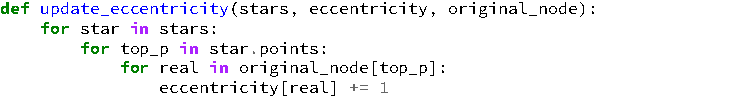
\includegraphics{assets/tmp-code/update_eccentricity.pdf}
    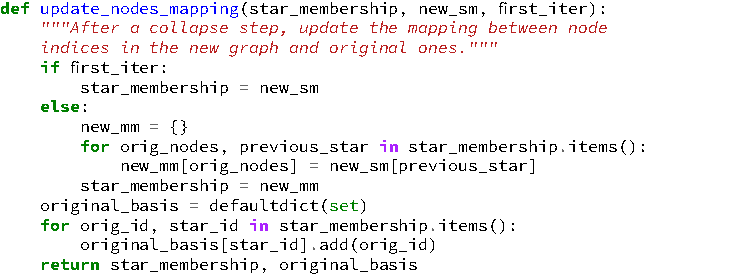
\includegraphics{assets/tmp-code/update_nodes_mapping.pdf}
    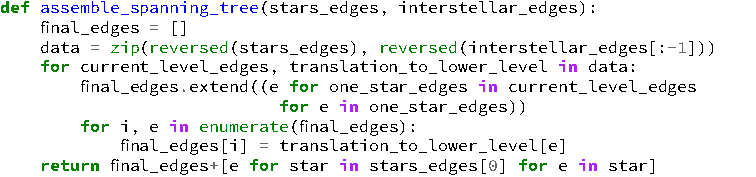
\includegraphics{assets/tmp-code/assemble_spanning_tree.pdf}
	\end{algorithmic}
\end{algorithm}

As described in \autoref{alg:gtx}, at every collapse level, we first extract stars from the current
graph (line 5), then update the eccentricity and node mappings (lines 7--8) and finally collapse the
graph (line 9). We perform these operations until there are no edge connecting stars anymore. At
this point, we revisit every outer edges to build the spanning tree (line 13).

\begin{prop}
  \label{prop:gtx_correct}
  For any connected graph $G_0$, \gtx$(G_0)$ terminates after $K\leq |V_0|$ iterations. Furthermore,
  it runs in $O(K|E_0|)$ time and returns a spanning tree of $G_0$.
\end{prop}
We will need the following lemma.
\begin{lemma}
  \label{lem:gtx_stay_connected}
  If $G_0$ is connected, then any subsequent graph $G_t,\, t \leq K$ is also connected.
\end{lemma}
\begin{proof}
 Suppose not and assume, to the contrary, that there exists at least one (or more) disconnected
 graph in $\{G_t\}_{t=1}^K$ and let $t_0$ be the smallest index such that $G_{t_0}$ is disconnected.
 Then there exist two nodes $s_u$ and $s_v$ in $V_{t_0}$ with no path between them in $E_{t_0}$.
 Letting $\mathcal{U}, \mathcal{V} \subset V_{t_0-1}$ be respectively the nodes forming stars $u$
 and $v$, this implies there is no path between nodes in $\mathcal{U}$ and nodes in $\mathcal{V}$.
 However, $G_{t_0-1}$ is connected by hypothesis, which leads to a contradiction.
\end{proof}

\begin{proof}[Proof of \autoref{prop:gtx_correct}]
  Let us first show that \gtx{} terminates in less than $|V_0|$ iterations. This follows from the
  fact that every time we collapse the graph $G_t$, we strictly reduce the number of nodes. Indeed,
  according to \autoref{lem:gtx_stay_connected}, $G_t$ is connected so at least two nodes of $V_t$
  are joined by an edge and will form a star, \ie{} a single node. We can thus claim that $|V_{t+1}| <
  |V_t|$. Note also that for all $t$, $|V_t| > 0$ and that when $|V_t|=1$, \extractStar{} creates a
  singleton and \collapseStar{} does not return any outer edges so \gtx{} finishes, proving that the
  number of iterations $K$ satisfies $K \leq |V_0|$.

 Then we analyze the time complexity. We already now that during the \tth{} iteration,
 \extractStar{} and \collapseStar{} take time $O(|E_t|)$. We only provide the actual python code
 instead of pseudo code for the remaining functions since they do not present any relevant
 algorithmic aspect. However, we can say that \textsc{Update-Eccentricity} and\marginpars{We can get
 rid of this $O(|V_0|)$ at each iteration by ignoring eccentricity and taking a random edge between
 star, although it's difficult to tell how it would affect the quality of the resulting tree.}
 \textsc{Update-Nodes-Mapping} take $O(|V_0|)$ time since they go through every node of the original
 graph. Because $G_0$ is connected, $|V_0| \leq |E_0|$, and since for all $t$, $|E_t| \leq |E_0|$,
 we have that the \gtx{} inner loop takes $O(K|E_0|)$ time. Finally, since
 \textsc{Assemble-Spanning-Tree} goes again through every edge visited at every collapse step, it
 also takes $O(K|E_0|)$ time, which is thus the overall complexity of the \gtx{} algorithm.


  Finally we prove that \gtx{} indeed returns a spanning tree of $G_0$. Specifically, we show that
  by starting from $G_K$ and going in reverse order, we build a spanning tree $T_t$ of every $G_t$,
  including eventually $G_0$. This process is illustrated on \autoref{fig:gtx_spanning_tree} and
  works as follow: when moving from $G_{t+1}$ to $G_t$, we expand the nodes of $G_{t+1}$ into star
  of nodes of $V_t$ and update all the outer edges we met so far to have their endpoints in $V_t$.
  These outer edges are exactly $T_{t+1}$ and by translating them into $E_t$ and adding the inner
  star edges of $G_t$, we build $T_t$. $G_K$ consists of a single node with no edges so we have
  trivially that $T_K$ = $G_K$. Then, assume we have a spanning tree $T_{t+1}$ of $G_{t+1}$, so that
  all nodes in $V_{t+1}$ are connected without cycle. Expanding each node of $V_{t+1}$ into a star
  of $V_t$ nodes ensures that the spanning property is preserved since each node of $V_t$ is covered
  by construction. Those stars are also without cycle by construction. The second step, translating
  the existing edges of $T_{t+1}$, only connects nodes belonging to different stars and because
  those edges were cycle free in $G_{t+1}$, this remains the case in $G_t$. Therefore we have build
  a spanning tree $T_t$ of $G_t$. By repeating this procedure, the \gtx{} algorithm eventually
  builds a spanning tree of $G_0$.
\end{proof}
\vspace{-2\baselineskip}
\begin{figure*}[h]
  \centering
	\begin{subfigure}[b]{37mm}
    \centering
		\includegraphics[width=\textwidth]{assets/tikz/gtx_st_g3_tikz.pdf}
		\caption{Spanning tree of $G_3$}\label{fig:gtx_spanning_tree_3}
	\end{subfigure}~
	\begin{subfigure}[b]{45mm}
    \centering
		\includegraphics[width=\textwidth]{assets/tikz/gtx_st_g2_tikz.pdf}
		\caption{Spanning tree of $G_2$}\label{fig:gtx_spanning_tree_2}
	\end{subfigure}~
	\begin{subfigure}[b]{49mm}
    \centering
		\includegraphics[width=\textwidth]{assets/tikz/gtx_st_g1_tikz.pdf}
		\caption{Spanning tree of $G_1$}\label{fig:gtx_spanning_tree_1}
	\end{subfigure}~
	\begin{subfigure}[b]{53mm}
    \centering
		\includegraphics[width=\textwidth]{assets/tikz/gtx_st_g0_tikz.pdf}
		\caption{Spanning tree of $G_0$}\label{fig:gtx_spanning_tree_0}
	\end{subfigure}~
  \caption{Unfolding stars to recover spanning trees}
  \label{fig:gtx_spanning_tree}
\end{figure*}

The bound of \autoref{prop:gtx_correct} amounts to $O(|V_0||E_0|)$, which we believe is overly
pessimistic. First because we expect the number of nodes to decrease by more than one at each step,
maybe leading to only $O(\log |V_0|)$ iterations. More importantly, instead of bounding
$\sum_{t=0}^K |E_t|$ by $K|E_0|$, we hope to show that $E_{t+1} = rE_t$ with $r<1$ so that this sum
is $O(|E_0|)$.

\paragraph{Example of \gtx{}}
\label{par:exemple_of_gtx}

We illustrate the operation of the \gtx{} algorithm on a small (and somewhat contrived) example.
Let us start with the initial graph $G_0$ depicted in \autoref{fig:gtx_eccentricity}
\vpageref{fig:gtx_eccentricity} and initialize
the eccentricity of all nodes to $0$. When running \extractStar{}, we see that the maximum degree is
$4$, achieved at nodes $\{1, 6, 11, 16, 21, 26, 31, 36, 41\}$. For the sake of simplicity, assume
nodes are picked according to their index. First, node $1$ forms the star $\starone{1}$ with
peripheral nodes $2$, $3$, $4$ and $5$. This increments the eccentricity of those peripheral nodes
by $1$. Then node $6$ forms its star $\starone{2}$ with $7$, $8$, $9$ and $10$. The process
continues until node $41$ is chosen to be the center of star $\starone{9}$, at which point the
max-priority queue has been exhausted and \extractStar{} finishes.

\begin{figure}[htbp]
  \centering
  \includegraphics[width=0.78\linewidth]{tikz/gtx_eccentricity_tikz.pdf}
  \caption[The hierarchical structure of stars created by \gtx{}]{%
    The execution of the \gtx{} algorithm. The original graph is made of the solid and dashed edges
    connecting the nodes labeled by their index. Edges forming the final spanning tree are solid
    while the others are dashed. Their colors indicate at which iteration they were chosen to be inside a
    star. The four shades of gray, from white to dark gray
    denote increasing node eccentricity (as computed at the end of the algorithm). The \ith{} star
    created during the \jth{} iteration of the algorithm is denoted $S_i^j$. Refer to the main text
    for the complete description of the execution.}
  \label{fig:gtx_eccentricity}
\end{figure}

\begin{figure}[bthp]
  \centering
  \begin{subfigure}[b]{0.47\textwidth}
    \centering
    \includegraphics[height=5cm]{tikz/gtx_run_level1_tikz}
    \caption{Resulting graph after the first iteration}\label{fig:gtx_run1}
  \end{subfigure}~
  \begin{subfigure}[b]{0.47\textwidth}
    \centering
    \includegraphics[height=2.2cm]{tikz/gtx_run_level2_tikz}
    \caption{Resulting graph after the second iteration}\label{fig:gtx_run2}
    \vspace{\baselineskip}
    \includegraphics[height=2.2cm]{tikz/gtx_run_level3_tikz}
    \caption{Resulting graph after the third iteration}\label{fig:gtx_run3}
  \end{subfigure}~
  \caption{The other iterations of \gtx{}}\label{fig:gtx_run}
\end{figure}

We then call \collapseStar{}. This will connect all possible pairs of star. For instance, the edge
between nodes $19$ and $29$ leads to the edge between $\starone{4}$ and $\starone{6}$. This is
actually the only possible edge between $\starone{4}$ and $\starone{6}$.  Consider on the other hand
the case of edges $(2, 6)$ and $(2, 9)$. They both connect $\starone{1}$ and $\starone{2}$. Yet at
this point of the algorithm, the eccentricity of node $2$ is $1$, the eccentricity of node $6$ is
$0$ and the eccentricity of node $9$ is $1$. The edge $(2, 6)$ has therefore the smallest total
eccentricity and is chosen to connect $\starone{1}$ and $\starone{2}$. The full result of the
\collapseStar{} procedure is $G_1$, which can be seen on \autoref{fig:gtx_run1}.

We now run \extractStar{} on $G_1$. Because all nodes have degree $2$, they could all be chosen to
be the center of a star yet we again they are picked according to their index and therefore we
choose $\starone{1}$ to be the center of the star $\startwo{1}$ with peripheral nodes $\starone{2}$
and $\starone{3}$. The original nodes belonging to those peripheral stars (nodes $4$ to $15$) have
their eccentricity incremented by $1$. The next node with highest degree in $G_1$ is now
$\starone{4}$, which forms a star with $\starone{5}$ and $\starone{6}$. This choice means that nodes
$21$ through $30$ have their eccentricity incremented by $1$. Finally, $\starone{7}$ forms the last
star with $\starone{8}$ and $\starone{9}$. Then \collapseStar{} connects the resulting three stars,
and this time there is only a single choice between each pair of stars, leading to the graph $G_2$
showed in \autoref{fig:gtx_run2}

The action of \extractStar{} on $G_2$ is quite simple, because there is only one star that can be
created, so let say we choose $\startwo{1}$ as its center, with $\startwo{2}$ and $\startwo{3}$ as
peripheral nodes. This increases the eccentricity of their underlying $G_0$ nodes by $1$ (namely
nodes $16$ to $45$). Because there is only one star $\starthree{1}$ left, \collapseStar{} returns
$G_3$ showed in \autoref{fig:gtx_run3} and an empty list of outer edges, meaning that the inner loop
of \gtx{} is finished and we can go through every edges we chose between stars at every level to
recover the final spanning tree, a process illustrated in \autoref{fig:gtx_spanning_tree}
\vpageref{fig:gtx_spanning_tree}. For completeness, we can also look at the edges which are not part
of the spanning tree and therefore contribute to the stretch of the tree. In that case the average
stretch is $7$, as showed in \autoref{tab:gtx_example_stretch}.

\begin{table}[htpb]
  \centering
  \caption{Stretch of the example tree}
  \label{tab:gtx_example_stretch}
  \begin{tabulary}{\linewidth}{lLr}
    \toprule
    test edge & path in the tree & length \\
    \midrule
    $2,9$   & $2$--$6$--$9$                       & $2$ \\
    $3,12$  & $3$--$1$--$4$--$14$--$11$--$12$     & $6$ \\
    $13,29$ & $13$--$11$--$15$--$26$--$29$        & $4$ \\
    $20,24$ & $20$--$16$--$17$--$23$--$21$--$24$  & $5$ \\
    $25,42$ & $25$--$21$--$23$--$17$--$16$--$19$--$29$--$26$--$15$--$11$--$14$--$4$--$1$--$2$--$6$--$8$--$37$--$36$--$39$-- $32$--$31$--$35$--$43$--$41$--$45$ & $24$ \\
    $33,38$ & $33$--$31$--$32$--$39$--$36$--$38$  & $5$ \\
    $34,43$ & $34$--$31$--$35$--$43$              & $3$ \\
    \bottomrule
  \end{tabulary}
\end{table}

\paragraph{Number of iterations needed}\label{par:number_of_iteration}%

\textcolor{red}{\LARGE Draft}

A crucial quantity of the \gtx{} algorithm, both in terms of complexity and resulting stretch, is
the number of collapses $K$ needed before termination. While this is still elusive to express in the
general case, let us first look at some simple cases. For instance, a very sparse example of graph
is the line graph. While it is already a tree, let us look how the \gtx{} algorithm operates on it.
Say we have $n$ nodes and $m$ edges in that line. Here, a star is made at most of three
consecutive nodes. In the worst case, centers will be chosen such that we have a succession of three
and two nodes stars, as in \autoref{fig:gtx_line_graph}.%
\begin{marginfigure}
  \centering
  \includegraphics[width=0.9\linewidth]{assets/tikz/gtx_line_tikz.pdf}
  \caption{A line graph with stars in blue}
  \label{fig:gtx_line_graph}
\end{marginfigure}
This will results in $\nicefrac{2n}{5}$ stars, which is less than half of $n$ and because in that
case $n=m+1$, \gtx{} will finish after $O(\log m)$ iterations. Note that a barbell graph (two
cliques connected by a line) would requires a number of iterations logarithmic in the length of that
central line, despite having many more edges. This suggests unsurprisingly that the diameter of the graph
could be a good parameter to quantify the number of iterations needed. Indeed, take a tree and consider
the length $p$ of its longest path from the root to a leaf. By a similar argument as the one used in
the line case, it seems \gtx{} will terminate after $O(\log p)$ iterations.

\iffalse
While all $G_t$ are connected according to \autoref{lem:gtx_stay_connected}, it might happen during
the execution of \extractStar{} that%
\begin{marginfigure}
  \centering
  \includegraphics[width=0.95\linewidth]{assets/tikz/gtx_singleton_tikz.pdf}
  \caption{The formation of a singleton star}
  \label{fig:gtx_singleton}
\end{marginfigure}
the degree of a node $u$ drops to zero because all of its neighbors were claimed by the
periphery of previous stars. Such a node then forms a \emph{singleton star}, as illustrated in
\autoref{fig:gtx_singleton}, where after the creation of \starone{1} and \starone{2}, $c_3$ is the
single node of the third star \starone{3}.

Such singleton stars are problematic because when too many are created, we can end up having
$|V_{t+1}|$ almost as large as $|V_t|$. Consider for instance the graph $G_t$ at the top of
\autoref{fig:gtx_manysingles} (which is actually a tree). It has of order $k^3$ nodes and because
all nodes at level 2 will be selected as center of their star, the graph $G_{t+1}$ (showed at the
bottom of \autoref{fig:gtx_manysingles}) also have around $k^3$ nodes, meaning that
$\frac{|V_{t+1}|}{|V_t|}$ tends to $1$ as $k$ goes to infinity. This is because
$k\left(k(k+1)\right)$ singleton stars were created. Let us denote the fraction of singleton stars
over the total number of nodes by $\alpha$. In that case,
$$\alpha = \frac{k\left(k(k+1)\right)}{1+k+k(k+1)+k^2(k+1)}
= 1 - \frac{1+2k+k^2}{1+2k+2k^2+k^3}
= 1 - \frac{1+k}{1+k+k^2}$$
We will now see that when so many singleton stars are created at one iteration, the next iteration
greatly reduces the number of nodes so that over the course of two iterations, we have the following
result:
{\color{blue}{\large the following is actually incorrect but I leave it for now for illustration
purpose}

\begin{lemma}
  \label{lemma:gtx_lessnodes}
  During the execution of the \gtx{} algorithm, for all $0\leq t \leq K-2$, $|V_{t+2}| \leq
  \frac{2}{3}|V_t|$.
\end{lemma}
\begin{marginfigure}
  \centering
  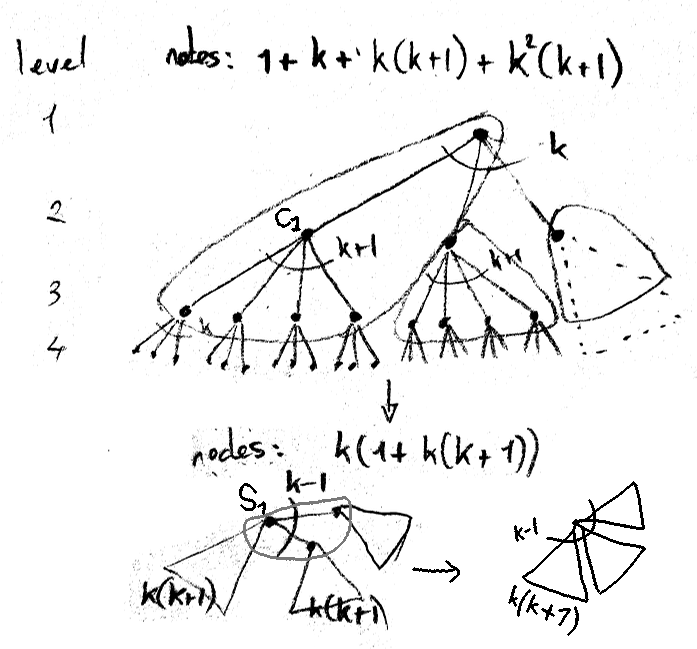
\includegraphics[width=\linewidth]{assets/raw/lots_of_singletons_bw.png}
  \caption{A case were too many singletons \enquote{waste} one iteration of \gtx{}}
  \label{fig:gtx_manysingles}
\end{marginfigure}
\begin{proof}
  Say that at iteration $t$ of \gtx{}, we have $n_t$ nodes and assume a fraction $\alpha$ of them
  will form singleton stars during the \tth{} iteration. This means there will be at most $\frac{1-\alpha}{2}n_t$
  \emph{proper} stars, because such stars are made of at least two nodes. Now fix a constant
  $\lambda \in (0,1)$, for instance $\lambda = \nicefrac{9}{10}$. If $\alpha \leq \lambda$, $n_{t+1}
  \leq (\frac{1-\alpha}{2} + \alpha)n_t = \frac{1+\alpha}{2}n_t$ and $\frac{1+\alpha}{2}n_t \leq
  \frac{1+\lambda}{2}n_t = \frac{19}{20}n_t$ so we get a
  constant rate reduction of the number of nodes. On the other hand, if $\alpha > \lambda$, we could
  be in the situation of the previous example and have $\alpha$ be arbitrarily close to $1$. Then we
  only have a few proper stars and by construction, each singleton star is connected to least one proper star.
  In the worst case, those connections are uniform so that each of these proper stars has degree at least
  $\frac{\alpha n_t}{\frac{1-\alpha}{2}n_t} = \frac{2\alpha}{1-\alpha}$ which goes to infinity when
  $\alpha$ goes to $1$ and is greater than $18$ when $\alpha$ is greater than $\nicefrac{9}{10}$.
  \textbf{Even ignoring the fact that those proper stars are connected}, it follows that in the next
  iteration, the number of node will be reduced by the degree of those proper stars. Setting in the
  worst case $n_{t+1}=\frac{1+\alpha}{2}n_t$, we thus have $$n_{t+2} \leq
  \frac{n_{t+1}}{\frac{2\alpha}{1-\alpha}} = \frac{1-\alpha^2}{4\alpha}n_t$$
  \begin{marginfigure}
    \centering
    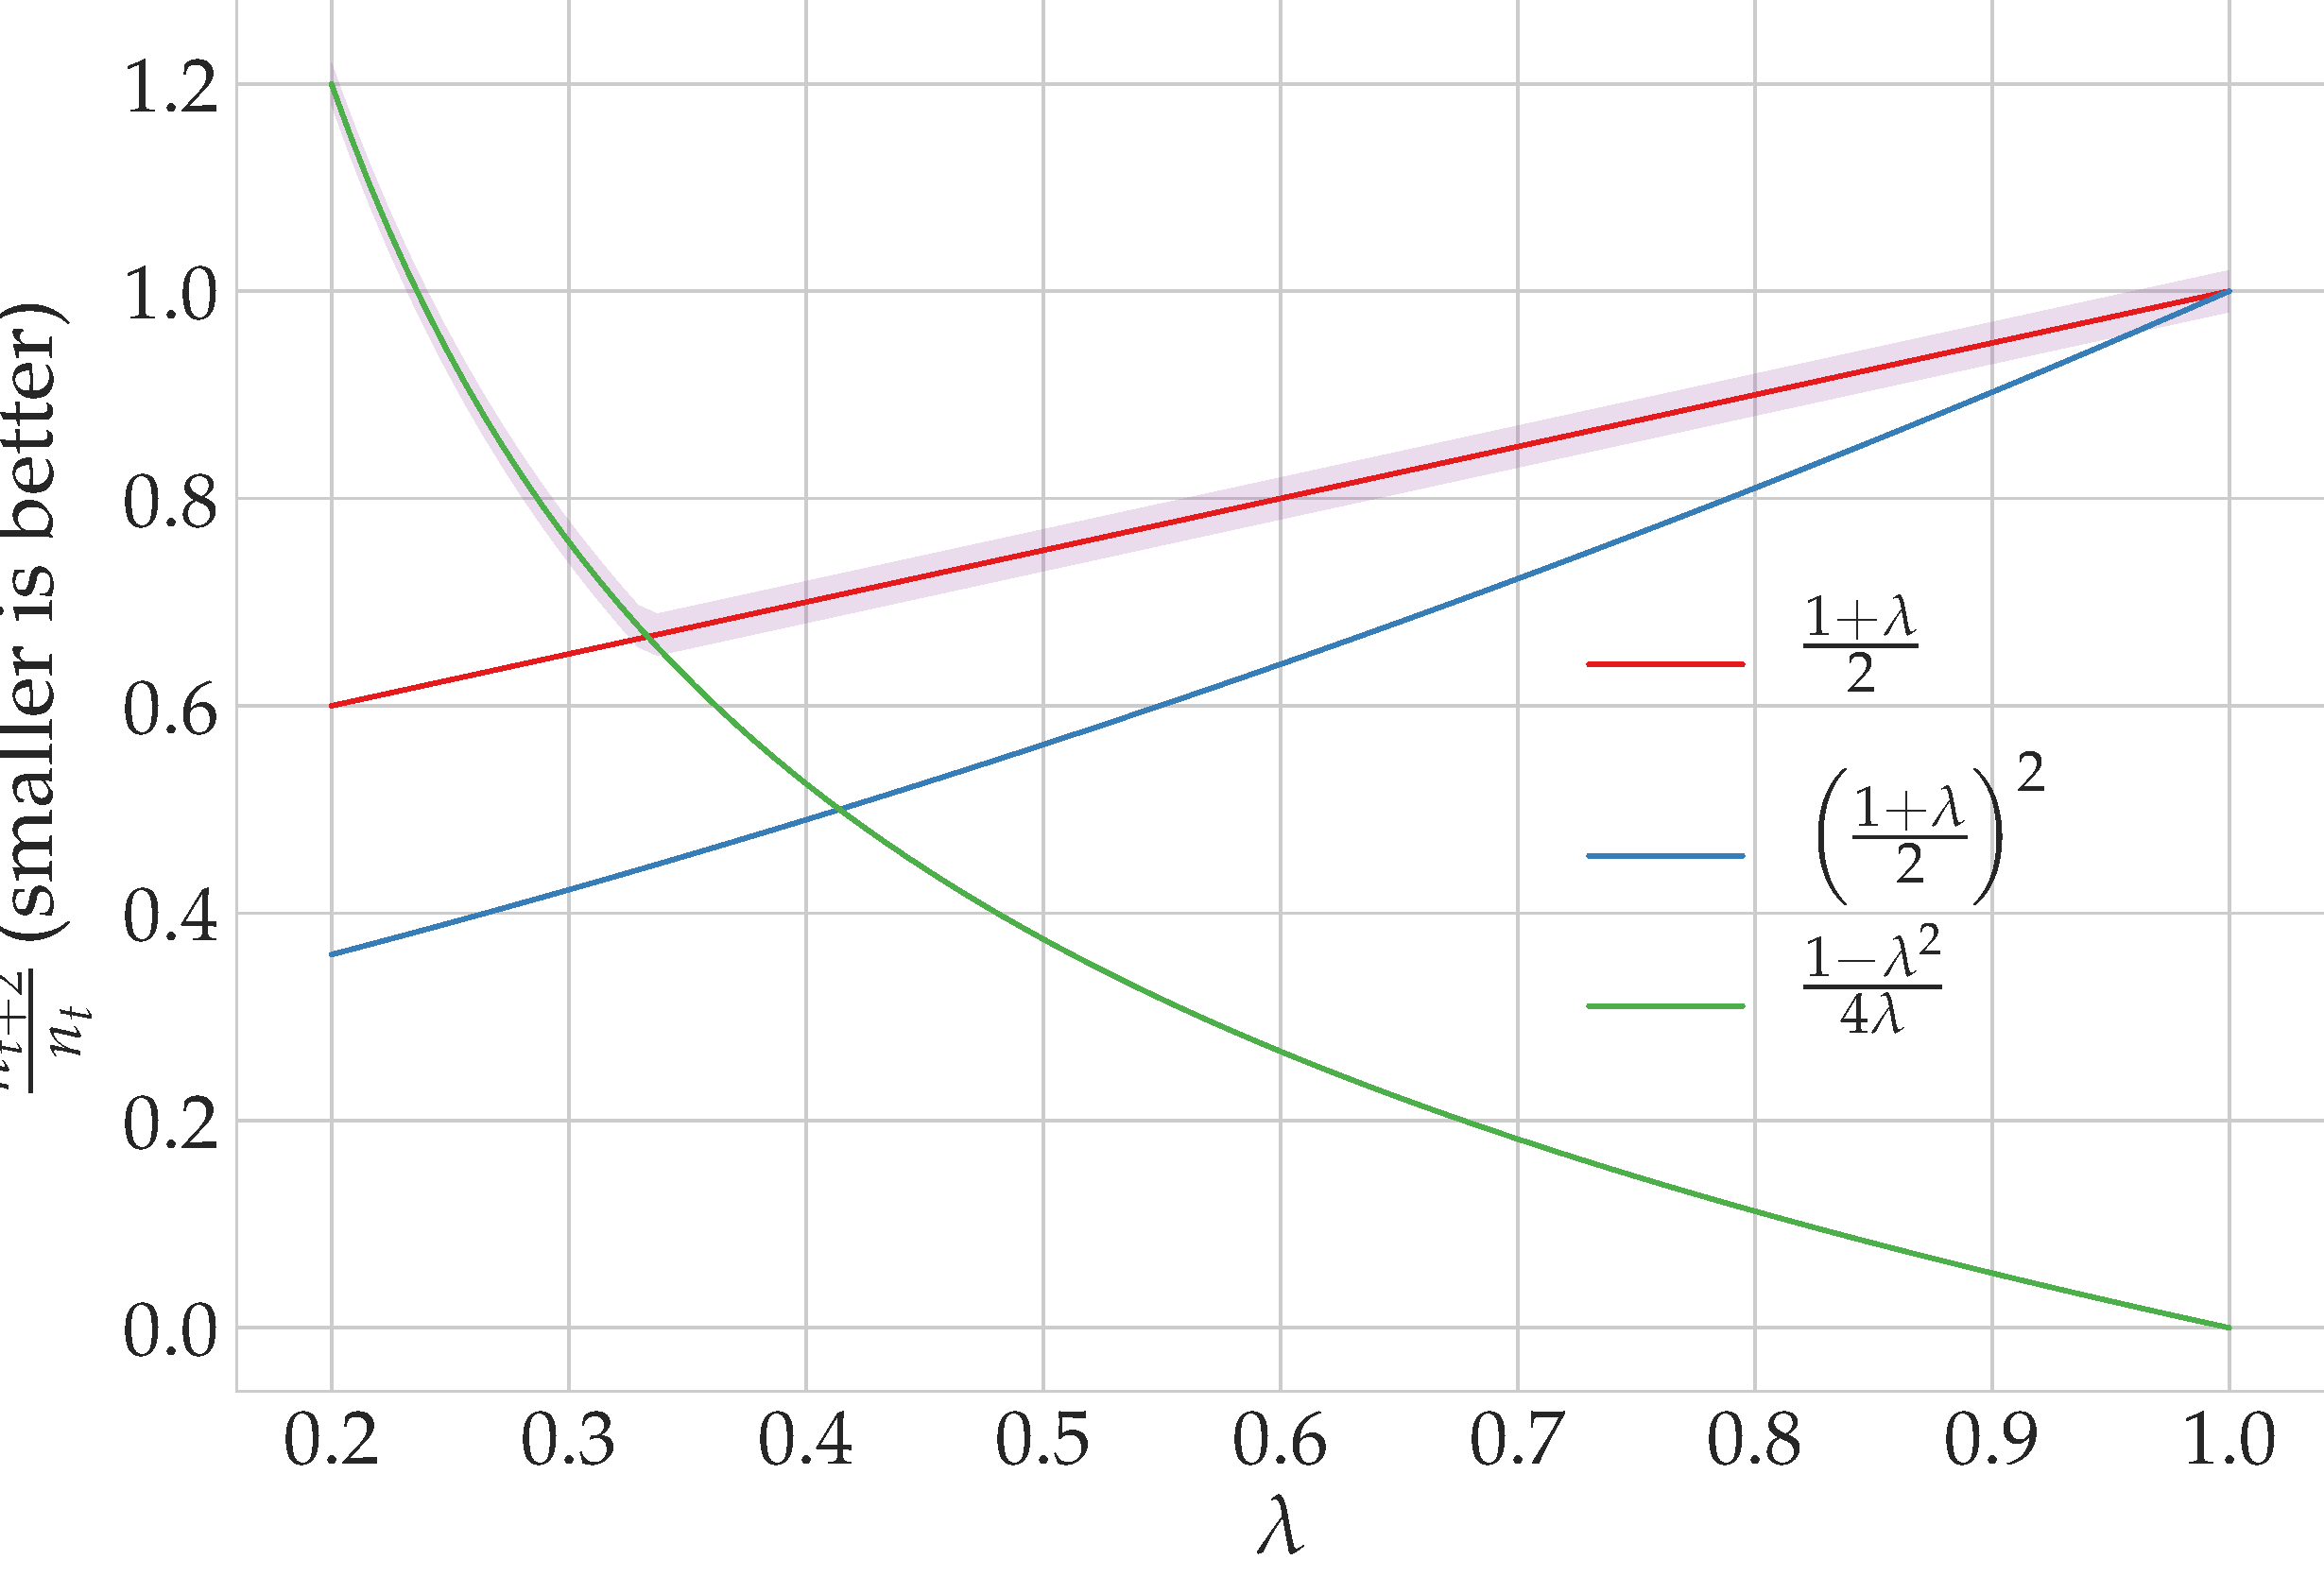
\includegraphics[width=\linewidth]{assets/tmp-code/gtx_reduc.pdf}
    \caption{The fraction of $n_t$ nodes remaining in $n_{t+2}$ for the three cases described in the
    main text.}
    % \label{fig:gtx_manysingles}
  \end{marginfigure}
  This defines three ways to go from $n_t$ to $n_{t+2}$: if the first iteration has $\alpha>\lambda$,
  then we just seen that in the worst case we have at least $n_{t+2}\leq
  \frac{1-\lambda^2}{4\lambda}n_t$; if the first iteration has $\alpha < \lambda$, then either the
  second also has  $\alpha < \lambda$ (in which case $n_{t+2}\leq
  \left(\frac{1+\lambda}{2}\right)^2n_t$) or the second has $\alpha>\lambda$ (in which case
  $n_{t+2}\leq \frac{1+\lambda}{2}n_t$). We can optimize over $\lambda$ by finding its value such
  that $\frac{1-\lambda^2}{4\lambda}=\frac{1+\lambda}{2}$, yielding $\lambda = \frac{1}{3}$. Then,
  in any event, $n_{t+2}\leq \frac{2}{3}n_t$ as claimed.
\end{proof}

From that we conclude that the number of iterations of the \gtx{} algorithm satisfies $K=O(\log
|V_0|)$.}
The problem is that we cannot ignore the fact that proper stars are connected, since one of them can
be connected to all others and have the highest degree. That proper star is then chosen as the first
center, all other proper stars become its periphery and all their attached singletons star remain
singleton stars at the next iteration. This actually what happens on \autoref{fig:gtx_manysingles},
an example where $|V_{t+2}| \sim |V_t| \sim k^3$. This could even be worse if proper stars are
connected in such a hierarchical way that singleton stars can survive for many iterations.


Here is another proof that does not work, where we study the diameter of the graph. Indeed, it is
initially bounded by the number of nodes $n$, and by the correctness of \gtx{}, it will be zero upon
termination. If we show that the diameter shrinks by a constant factor at each iteration, then we
can claim that \gtx{} terminates after a number of iterations logarithmic in $n$. For ease of
exposition, we instead prove equivalently that when going backward in time, the diameter expands at
least by a constant factor at each iteration. Let us denote by $\Delta_t$ the diameter of $G_t$ and
take any path of length $\ell \leq \Delta_t$ in $G_t$. Let $[s_1, s_2, \ldots, s_{\ell+1}]$ be the
nodes along this path, where the notation $s_i$ reflects the fact that these nodes were stars of
nodes in $G_{t-1}$. If we choose any $u,v \in V_{t-1}^2$ such that $u$ is in the star $s_1$ and $v$
is in the star $s_{\ell+1}$, then we can see on \autoref{fig:gtx_expand_path} that there exists a
path of length $2\ell -1$ between $u$ and $v$ in $G_{t-1}$.
{\color{blue}{\large The figure actually shows this is not always true.}
More generally, for any path of length
$\ell$ in $G_t$, there is a path of length $2\ell-1$ in $G_{t-1}$. In particular, for
$\ell=\Delta_t$, there is a path of length $2\Delta_t-1$ in $G_{t-1}$, from which we conclude that
$2\Delta_t-1\leq\Delta_{t-1}$, or equivalently $\Delta_t \leq
\frac{1}{2}\left(\Delta_{t-1}+1\right)$. One can then check by recurrence that $\Delta_t \leq
\frac{1}{2^t} \left(\Delta_0+2^t-1\right) \leq \frac{n}{2^t} + 1$.}

\begin{figure*}[htpb]
   \centering
   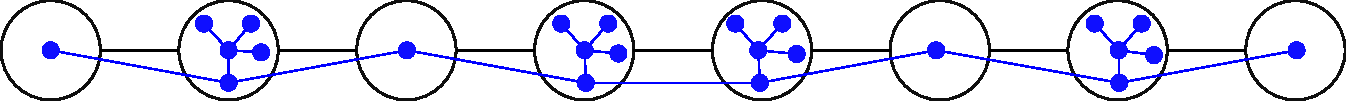
\includegraphics[width=\linewidth]{raw/expand_path.pdf}
   \caption[Star expansion of a path]{A path within $G_t$ in black, and the underlying graph
     $G_{t-1}$ in blue. In the worst case, the endpoints of the path in $G_{t-1}$ are at the
     periphery of the endpoint stars.  The intermediary nodes in $G_t$ could be proper or singleton
     star, but there cannot be two adjacent singleton stars.}
   \label{fig:gtx_expand_path}
\end{figure*}
\fi

\iffalse
We would like to prove a similar result on the edges so that the overall complexity of the
\gtx{} algorithm would be $O(|V_0|\log |V_0|+|E_0|)$. However, this does not follow directly from the
reduction of number of nodes. Indeed, we can have a situation where most of the edges of $E_t$ are
between the stars of $G_t$ and thus will remain in the next iteration. Still, we hope that
similarly to the previous proof, this high density of outer edges will lead to strong collapse in
the next iteration.

In the case no singleton are formed during one execution of \extractStar{}, the number of nodes is
reduced by at least a factor $2$ (because each star is made of at least two nodes). On the other hand, we can
construct a graph with singletons where the factor of reduction in number of nodes and edges can be
arbitrarily close to $1$. Consider \autoref{fig:gtx_noreduc}, where $c_1$ and $c_2$ have a degree
$p$ and their neighbors (in light gray) all have a degree $q$, which we can vary from $1$ to $p-1$.
At this step $t$, we thus have $|V_t| = 2(1+p)+pq$ and $|E_t| = 2(p+qp)$. Next we run \extractStar{}
and assume that we first extract the two stars centered in $c_1$ and $c_2$. This reduces the
effective degree of all the middle nodes (in dark gray) to $0$ and they thus form singletons, that
are all connected to the first two stars by \collapseStar{}. As a result, at step $t+1$ we have%
\begin{marginfigure}
  \centering
  \includegraphics[width=0.95\linewidth]{assets/tikz/gtx_noreduc_tikz.pdf}
  \caption{A case were too many singletons \enquote{waste} one iteration of \gtx{}}
  \label{fig:gtx_noreduc}
\end{marginfigure}
$|V_{t+1}| = 2 + pq$ and $|E_{t+1}| = 2pq$, so that
\begin{equation*}
\frac{|V_{t+1}|}{|V_t|} = \frac{pq+2}{p(q+2) + 2} \qquad \text{and} \qquad
\frac{|E_{t+1}|}{|E_t|} = \frac{2pq}{2p(q+1)} = \frac{q}{q+1}
\end{equation*}
When we let $p$ goes to infinity, setting $q=1$ makes $\frac{|V_{t+1}|}{|V_t|}$ tend to
$\nicefrac{1}{3}$ and $\frac{|E_{t+1}|}{|E_t|}$ to $\nicefrac{1}{2}$ while setting $q=p-1$ makes
both $\frac{|V_{t+1}|}{|V_t|}$ and $\frac{|E_{t+1}|}{|E_t|}$ tend to $1$. Note however that in both
cases, this is not really a problem because at the next iteration, there will be only two stars (one
of them will be a singleton). Is it always like that? In other words, can we have a situation where
a large number of singletons is carried over several consecutive iterations?
\fi

\paragraph{Variants of \extractStar{}}
\label{ssec:gtx_center_choice}

The execution of \extractStar{} is mainly deterministic, except for the fact the ties between nodes
with the same highest degree are broken arbitrarily. While this allows for an efficient
implementation, and simplify the analysis of the resulting sequence of stars and therefore the
induced spanning tree, in can be detrimental in an adversarial context, where we could end up with a
tree forcing a lot of mistakes. We add an element of randomization to \extractStar{} by letting it
use of two optional arguments, a \emph{threshold function} $\tau$ or a \emph{degree function}
$\widetilde{d}$. Such functions modify the center sampling process in the following way:
\begin{itemize}%[nosep]
  \item if $n_{t,i}$ is the number of node remaining in $V_t$ before choosing the \ith{} center, choose
    a node \uar{} among those with a degree larger than $\tau(n_{t,i})$. The idea is to choose
    among a small set of high degree nodes, for instance by letting $\tau(n) = \sqrt{n}$. Note
    however we cannot guarantee there will always be nodes with degree above the threshold, in which
    case we default on the highest degree node
  \item if $\degr_i(u)$ is the degree of node $u$ before choosing the \ith{} center, choose node
    proportionally to $\widetilde{d}(\degr_i(u))$. Again, the degree function is designed so that it
    favors the selection of high degree nodes. For instance, one could use
    $\widetilde{d}(\degr_i(u)) = \degr_i(u)^2$.
\end{itemize}

These two variants are more time consuming because they require additional bookkeeping.
Therefore, we don't provide a full complexity analysis and only briefly sketch their implementations
here.\footnote{Although they are available online at
\nolinkurl{https://github.com/daureg/magnet/blob/master/veverica/}%
\{\href{https://github.com/daureg/magnet/blob/master/veverica/ThresholdSampler.py}%
{ThresholdSampler.py}, \href{https://github.com/daureg/magnet/blob/master/veverica/NodeSampler.py}%
{NodeSampler.py}\}.} For the threshold function, we
maintain two queues, $high$ and $low$, containing nodes whose degree is respectively above and below
the current threshold. We select a node \uar{} in $high$, remove the corresponding star from $G_t$,
recompute the new threshold and if necessary, move nodes which fell under the threshold from $high$
to $low$ and those who climb above the threshold from $low$ to $high$. For the degree function, we
can draw any node as center proportionally to its weight (where the weight of node $u$ is defined as
$d_f\left(\degr(u)\right)$). Yet we cannot use the standard method of computing the cumulative sum
of weights since some of them change at each iteration. Therefore, we construct a binary tree whose
leaves are the nodes of $V_t$ and where each tree nodes maintain the sum of weights in its left and
right subtrees. To sample, we draw a random number $r$ between $0$ and the total weight of the tree and
go down from the root to the leaf spanning the weight interval containing $r$.
When degrees are updated (or graph node removed), we update the weights along a path from the
corresponding leaves to the root of the tree.

A variant of the \gtx{} algorithm as a whole we did not explore so much in practice is its ability
to produce spanner by stopping early. Basically if we stop at iteration $t$, we output the graph
$G_t$ (which in general is not a tree) with its edges unfolded to lie in $E_0$. This corresponds to
a trade off between having more edges than $|V_0|-1$ but potentially making shorter connection and
thus having a lower stretch. This would also be interesting in the sign prediction setting. Assuming
the treewidth of $G_t$ is decreasing with $t$, maybe we could show there is \enquote{reasonable}
number of paths between $u$ and $v$, compute their parity and take a majority vote on the results.
